\begin{auf}
    646
\end{auf}
Ein waagrechter, $l=40 mm$ langer und $d=2mm$ dicker runder Kupferstab tritt
frei fallend und beidseitig geführt durch zwei senkrechte, elektrisch leitende Schienen von vernachlässigbarem ohmschen Widerstand in ein horizontales homogenes
Magnetfeld der Flussdichte $B=0.035T$ ein und durchquert dieses.
\begin{enumerate}
    \item[a] Aus welcher Höhe $h$ über dem oberen Rand des Magnetfeldes muss der Stab losgelassen werden, wenn er das Feld mit konstanter Geschwindigkeit	$v$ passieren soll?
    \item[b] Wie groß sind betragsmäßig die induzierte Spannung, der Strom, die Bremskraft und die im Stab umgesetzte elektrische Leistung? In welcher Richtung fließt der Strom? Daten von	Kupfer: $\varrho_m=8.96\cdot10^3\frac{kg}{m^3}$, $\varrho=1.78\cdot10^{-8}\Omega m$.
\end{enumerate}
\begin{figure}[h]
    \centering
    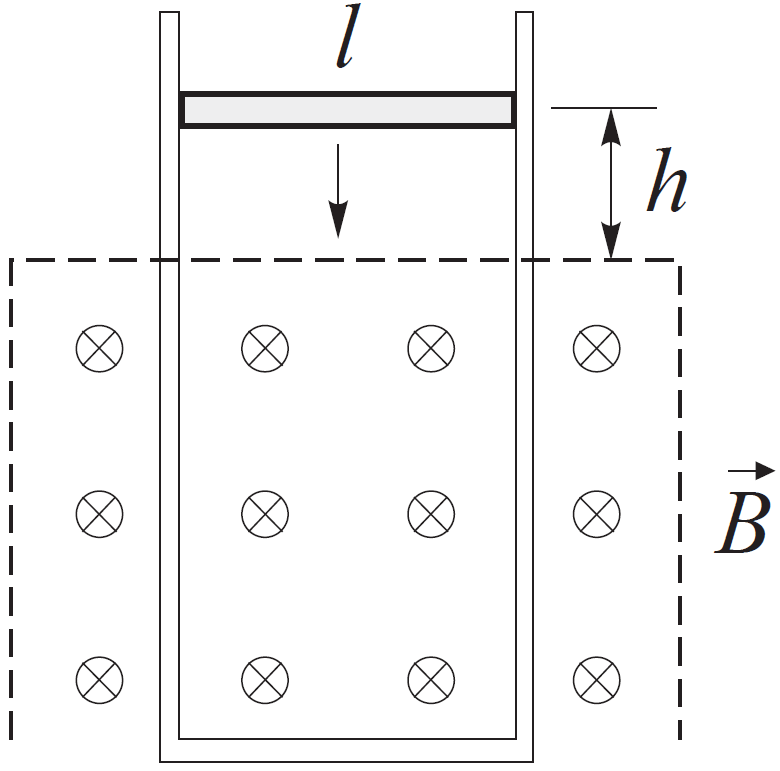
\includegraphics[height=5cm]{images/646_0.png}
    \caption{Versuchsaufbau Aufgabe 646}
\end{figure}